%%%%%%%%%%%%%%%%%%%%%%%%%%%%%%%%%%%%%%%%%%%%%%%%%%%%%%%%%%%%%%%%%%%%%%%%%%%%%%%%%%%%%%%%%%%%%%%%%%%
% Chapter 3 -> Single Multimodal Integration Problem
% Author: Mingbo Cheng
%%%%%%%%%%%%%%%%%%%%%%%%%%%%%%%%%%%%%%%%%%%%%%%%%%%%%%%%%%%%%%%%%%%%%%%%%%%%%%%%%%%%%%%%%%%%%%%%%%%
%\addbibresource{~/MEGA/MEGAsync/phd/thesis_Cheng/preamble/thesis.bib}
%\addbibresource{/home/mingbo/MEGAsync/phd/thesis_Cheng/preamble/thesis.bib}
\chapter{Single Cell Multimodal Trajectory Inference Problem}
\label{chapter:problem_TI}
\graphicspath{{chapter6/figs/}}

\subsection{Single Cell Multimodal Integration}
We will discuss the computational challenge of integrating single-cell multimodal data, provide an overview of current methods for the task, and outline our objectives for addressing the limitations present in existing computational approaches to single-cell multimodal integration.
\subsubsection{Challenge of Single Cell Multimodal Integration}
\label{background:sec2:challenge_integration}
Single-cell multimodal profiling represents a nascent field, and the integration of single-cell multimodal data, while several tools have been developed for this purpose, still poses challenges:

\begin{itemize}
	\item \textbf{Heterogeneous statistical properties:}
	Different modalities exhibit distinct statistical properties, presenting a challenge for the integration of single-cell multimodal data. For instance, the feature size of single-cell surface proteins is typically around 100, while single-cell RNA-seq and single-cell ATAC-seq have feature sizes of 20,000+ and 100,000+~(\fref{fig:modalities_differences}A). The sparsity levels of the feature matrices for different modalities also vary significantly. For example, there are more than 10\% non-zero entries for scRNA-seq data, whereas scATAC-seq data has less than 3\% non-zero entries~\citep{li2021chromatin}, and surface protein data has more than 70\% non-zero entries~(\fref{fig:modalities_differences}B). Moreover, the feature distributions significantly differ among distinct modalities~(\fref{fig:modalities_differences}C). The substantial differences between modalities present a significant challenge in deriving a unified latent space that effectively incorporates all features without losing valuable information.


	\item \textbf{Modality Compatibility:}
	Increasingly, new protocols are being developed to simultaneously measure features in the same single cell, such as open chromatin, gene expression, protein, and DNA methylation. The combinations of different modality types present a challenge for integration; Certain methods, such as scAI~\citep{jin2020scai}, are designed to handle only two modalities, while others, like Liger~\citep{kriebel2022uinmf}, are restricted to specific feature matrices.

	\item \textbf{Scalability:}
	As sequencing costs decrease and technologies improve, we anticipate that multimodal datasets will follow a similar trend as single-cell RNA sequencing~(scRNA-seq), where in less than ten years, the size of experiments increased from the order of tens to millions of cells~\citep{svensson2018exponential}. More efficient methods are needed, ones that require less memory and reduced running time.

	\item \textbf{Interpretability:}
	Interpretation of each component of the latent space is essential to understand the information it captured in the latent space, some methods like Seurat WNN~\citep{hao2021seurat4} only delivered a network for the integration. When associating molecular features with the latent space, it's better if the method is capable of interpreting each component using features from specific modalities, and most methods lack this ability.

	\item \textbf{Removal of batch effects}:
	In single-cell multimodal integration, addressing heterogeneous features across different modalities is crucial, and the challenge extends to mitigating batch effects arising from both biological and technical sources. Certain methods, such as scAI~\citep{jin2020scai}, might be limited in their ability to incorporate external batch correction techniques, potentially leading to confounding results from combined batches and biological variations.

	\item \textbf{Validation}
	Evaluating the outcomes of data integration presents a significant challenge. In practice, there is no definitive ground truth, necessitating an evaluation based on downstream analysis tasks, such as assessing clustering agreement with true labels. However, these true labels, often annotations from a study, may introduce noise or inaccuracies in cell type identification. Therefore, a thorough validation should be applied to comprehensively assess the effectiveness of a method.

  \item \textbf{Execessive Presumption}
  Most methods either assume a specific data distribution or involve fitting the model with several parameters, requiring prior knowledge that may not be universally applicable. For example, Seurat WNN requires inputting the number of neighbors and scaling factor for the neighborhood, and MOFA involves several hyperparameters for model regularization, detection of number of factors and learning rates. Moreover, MOFA requires manual selection of informative components for downstream analysis after obtaining the latent components. A method is needed to automatically identify the most important shared information across different modalities.

\end{itemize}

\begin{figure}[!ht]
	\centering
	\includegraphics[width=0.95\textwidth]{feature_statistic/fig}
	\vspace{0.1cm}
	\caption[features characteristics comparison showing the challenge of multimodal integration.]{Illustration of six single-cell multimodal data. A) Number of features in scRNA, scATAC and scADT modalities. B) Percentage of zero entries in the three modalities, C) Element counts percentages in different modalities for the six single cell multimodal data.}
	\label{fig:modalities_differences}
\end{figure}

\subsubsection{Computational Methods for Single Cell Multimodal Integration}
\label{background:sec2:integration}
The challenges discussed in \sref{background:sec2:challenge_integration} regarding the integration of single-cell multimodal data pose difficulties in developing an efficient and effective integration method.

\begin{table}[!ht]
	\small
	\centering
	\begin{tabular}{llllll}
		\toprule
		Name & algorithm & modality types & \#modalities & Reference \\
		\midrule
    DIABLO & PLS-DA & universal & any & \cite{singh2019diablo}\\
    Liger & NMF & shared-features& 2 & \cite{kriebel2021nonnegative} \\
		MOFA   &  Matrix Factorization & universal & any &  \cite{argelaguet2020mofa+} \\
		Schema & Metrics learning  & universal & any & \cite{singh2021schema} \\
    scAI & Matrix Factorization & scRNA,scATAC & 2 & \cite{jin2020scai}\\
		Seurat WNN	 & WNN & universal & any & \cite{hao2021seurat4} \\
		\bottomrule
	\end{tabular}
	\vspace{0.1cm}
	\caption[Overview of computational integration methods]{Overview of computational integration methods.}
	\label{tab:methods_integration_overview}
\end{table}

Several methods have been developed to address this task, and we will now review the computational single-cell multimodal integration methods available in the literature. These methods can be classified into four groups based on the techniques they employ. The first group encompasses matrix factorization, which breaks down the multimodal count matrix into the product of two matrices. One matrix contains the latent factors representing the features, while the other incorporates the cells embedded in the latent factor space~(e.g., MOFA, scAI, Liger). The second group endeavors to construct a weighted nearest network that captures common information across all modalities~(e.g., Seurat WNN). The third group seeks to maximize the covariance or correlation between two modalities~(e.g., DIABLO, Symphony). The fourth group employs metric learning to reweigh modality features by maximizing their agreement with other modalities~(Schema). \tref{tab:methods_integration_overview} summarizes the characteristics of each method.
 \begin{figure}[!h]
  	\centering
  	\includegraphics[width=0.9\textwidth]{Alg/fig}
  	\vspace{0.1cm}
  	\caption[Illustration of competing integration competing method.]{\textbf{Illustration of competing integration competing method.} \emph{Source~\cite{kriebel2022uinmf}}~(modified to fit thesis format and/or clarify key points)
  }
  	\label{fig:Alg}
 \end{figure}


\begin{description}
  \item[DIABLO]
  Data Integration Analysis for Biomarker discovery using Latent cOmponents~(DIABLO) is a generalization of sGCCA~\citep{tenenhaus2014variable}, which is a multivariate extension of canonical correlation analysis~(CCA). For $Q$ normalized and centered data matrices $X^1, \cdots, X^Q$ of dimensions $N\times D_q$, where $N$ denotes the number of cells and $D_q$ denotes the number of features. DIABLO aims to find a set of $H$ linear combinations of the $Q$ data matrices that are maximally correlated. The linear combinations are defined as:
  \begin{equation}
  \begin{aligned}
  	\underset{a_h^{(1)},\cdots,a_h^{(Q)}}{\max} \sum_{i,j=1, i\neq j}^Q c_{i,j} \text{cov}(X_h^{(i)} a_h^{(i)}, X_h^{(j)} a_h^{(j)}),\\
  	s.t. \|a_h^{(q)}\|_2 = 1, \text{ and } \|a_h^{(q)}\|_1 \leq \lambda^{(q)}, \text{for all} 1\leq q \leq Q.
  \end{aligned}
  \end{equation}
  Where $a_h^{(q)}$ is the variable coefficient vector for the $h$-th linear combination of the $q$-th data matrix, and $c_{i,j}$ is the weight of the correlation between the $i$-th and $j$-th data matrices. The first constraint is to normalize the linear combination, and the second constraint is to sparsify the linear combination. DIABLO solves the optimization problem by iteratively updating the $a_h^{(q)}$ and $c_{i,j}$ until convergence.


 \begin{figure}[!h]
  	\centering
  	\includegraphics[width=0.6\textwidth]{Alg_Liger/fig}
  	\vspace{0.1cm}
  	\caption[Illustration of Liger integration competing method.]{\textbf{Illustration of Liger integration competing method.} Liger Schematic representation of the matrix factorization strategy~(top) and the formulation of the optimization problem~(bottom). The introduction of a factor matrix $U_i$ enables the utilization of unshared features in joint matrix factorization. Each dataset~($E_i$) undergoes decomposition into shared metagenes~($W$), dataset-specific metagenes constructed from shared features~($V_i$), unshared metagenes~($U_i$), and cell factor loadings~($H_i$). The inclusion of the U matrix enables unshared features occurring in only one dataset to contribute to the resulting integration. \emph{Source~\cite{kriebel2022uinmf}}~(modified to fit thesis format and/or clarify key points)
  }
  	\label{fig:Alg_Liger}
 \end{figure}

  \item[Liger]
  Linked Inference of Genomic Experimental Relationships~(Liger)~\citep{kriebel2022uinmf} implemented UINMF algorithm, which uses iterative Non-negative Matrix Factorization~(iNMF) to learn a common latent space across multiple modalities~(\fref{fig:Alg_Liger}). It allows the inclusion of both shared and unshared features across modalities to learn a common latent space. They incorporate intergenic peaks from snATAC-seq data and additional genes not measured in all datasets. For each data set $E^1, E^2, \cdots, E^n$, Liger first normalizes the data, and selects $m$ variable genes~(shared across all datasets), and $z_i$ variable features, such that after scaling $E^i \in R_{+}^{(m+z_i)\times n_i}\ (i=1,\cdots,N)$. Given $K$ and $\lambda_i$, the objective function is:
  \begin{equation}
	  \underset{H^i\geq 0,W\geq 0, V^i\geq 0, U^i \geq 0}{\arg\min} \sum_i^{d}\Big\| (E^i P^i) - H^i \big((W 0) + (V^i U^i)\big)\Big\|_{F}^2 + \lambda_i\sum_i^d\Big\|H^i(V^i U^i)\Big\|_{F}^2
  \end{equation}
  Liger uses coordinate block descent~(BCD) to solve the optimization problem, which derives the parameters into blocks and finds the optimal solution for each block iteratively.


\begin{figure}[!h]
  	\centering
  	\includegraphics[width=0.65\textwidth]{Alg_MOFA/fig}
  	\vspace{0.1cm}
  	\caption[Illustration of MOFA integration competing method.]{\textbf{Illustration of MOFA integration competing method.} MOFA takes $m$ data matrices as input $Y_1, \cdots Y_m$, one or more from each data modality, with co-occurrent samples but features that are not necessarily related and that can differ in numbers. MOFA decomposes these matrices into a matrix of factors~($Z$) for each sample and $m$ weight matrices, one for each data modality~($W_1,\cdots, W_m$) where white cells in the weight matrices correspond to zeros~(i.e., inactive features). The cross symbol in the data matrices represents missing values. \emph{Source~\cite{tewari2017mofa}}~(modified to fit thesis format and/or clarify key points)
  }
  	\label{fig:Alg_MOFA}
\end{figure}
 
  \item[MOFA]
  Multi-Omics Factor Analysis+~(MOFA+)~\citep{argelaguet2020mofa+} uses Bayesian group factor analysis and variational inference to decompose individual modalities simultaneously by estimating a common latent factor matrix $Z$, as well as the weights for the transformation of the modalities to the latent space~(\fref{fig:Alg_MOFA}). MOFA+ includes a procedure to determine the optimal number of factors~(dimension of the latent space) and has several hyper parameters for model regularization, detection of number of factors and learning rates. Specifically, it decomposes simultaneous multimodal of $M$ data matrics $Y^1, \cdots, Y^M$ of dimensions $N\times D_m$, where $N$ denotes the number of cells and $D_m$ denotes the number of features, $G$ is the number of sample groups, and $N_g$ is the number of samples in the $g$th group and $K$ is the number of factors. The matrix decomposition is:
  \begin{equation}
  Y_{gm} = ZgW_m^{T} + \varepsilon_{gm},
  \end{equation}
  Where $Y_{gm}$ is the the matrix of observations for the $m$th data modality and the $g$th group, $Z_g$ is the matrix of latent factors for the $g$th group, $W_m$ is the matrix of weights for the $m$th data modality, and $\varepsilon_{gm}$ is the matrix of residuals. The latent factors $Z_g$ are shared across all modalities, while the weights $W_m$ are specific to each modality. %%TODO: the decomposition algorithm

\begin{figure}[!h]
  	\centering
  	\includegraphics[width=0.8\textwidth]{Alg_Schema/fig}
  	\vspace{0.1cm}
  	\caption[Illustration of Schema integration competing method.]{\textbf{Illustration of Schema integration competing method.} Schema explores metrics learning to re-weigh modality features through maximizing the agreement with other modalities. Specifically, it utilizes quadratic programming~(QP) to learn a scaling transformation $u$ for the primary matrix $X$ such that pairwise distances of the transformation $u * x_i$~(where $*$ is coordinate-wise multiplication, for each $x_i\in X$) are highly correlated in other modalities. \emph{Source~\cite{singh2021schema}}~(modified to fit thesis format and/or clarify key points)
 } 
  	\label{fig:Alg_Schema}
\end{figure} 

  \item[Schema]
  Schema~\citep{singh2021schema} applied metrics learning to reweigh modality features by maximizing the agreement with other modalities~(\fref{fig:Alg_Schema}). Specifically, it utilizes quadratic programming~(QP) to learn a scaling transformation $u$ for the primary matrix $X$ such that pairwise distances of the transformation $u * x_i$~(where $*$ is coordinate-wise multiplication, for each $x_i\in X$) are highly correlated other modalities. Specifically, it assumes $N$ observations across $r$ datasets $D_j$, where $j=1,\cdots,r$ and $D_j = \{x_i^{j}: i = 1,2,\cdots,N\}$ contains data for each observation. First, it refers $D_1$ as the primary modality and $D_2,\cdots,D_r$ as the secondary modalities. Next, it computes the pairwise distances $\rho_1,\cdots,\rho_j$ for each modality $D_j$ where $\rho_j(x_n^{j}, x_m^{(j)})$ is the distance between observation $n$ and $m$ in $D_j$. Then, it aims to find a transformation $\Omega$ with $\Omega(D)$ generating a dataset $D^{*}$ such that the Euclidean metric $\rho^{*}$ on $D^{*}$ on $D^{*}$ aligns the various metrics. $\Omega$ is limited to be a scaling transformation $\Omega(D) = \{diag(u)x: x \in D\}$, where $u \in \mathbb{R}^{k}$ and $diag(u)$ is a $k\times k$ diagonal matrix with diagonal entries $u$. Then, the squared distance between points under the transformation is given by:
  \begin{equation}
  \rho^{*}(x_n, x_m) = \|diag(u)x_n - diag(u)x_m\|^2 = \|diag(w)(x_n - x_m)\|^2
  \end{equation}
  where $w$ is the element-wise square of u. The scaling transforms u acts as a feature-weighting mechanism to choose the features of $D_1$ that align the datasets best. Schema integrates between the metrics $\rho_j$ to learn a metric $\rho^{*}$ that aligns well with all of them. The correlation between $\rho^{*}$ and $\rho_j$ is measured by the Pearson correlation coefficient. And to tackle multiple modalities, Schema maximizes the sum of Pearson correlation between $\rho^{*}$ and all other modalities pairwise distances $\rho_2,\cdots,\rho_j$.
\begin{figure}[!h]
  	\centering
  	\includegraphics[width=0.55\textwidth]{Alg_scAI/fig}
  	\vspace{0.1cm}
  	\caption[Illustration of Seurat scAI integration competing method.]{\textbf{Illustration of Seurat scAI integration competing method.} scAI iteratively learns aggregated epigenomic profiles and low-dimensional representations from parallel scRNA-seq and scATAC-seq/single cell DNA methylation data. Input matrices consist of cells in rows and genes or loci in columns. The first step involves aggregating the epigenomic profile based on a randomly initiated cell-cell similarity matrix. In the second step, both transcriptomic and aggregated epigenomic data are concurrently decomposed into low-rank matrices, with gene, locus, and cell loading matrices indicating contributions for each factor. The third step computes a cell-cell similarity matrix based on the cell loading matrix. These steps iterate until a predefined stop criterion is met. \emph{Source~\cite{jin2020scai}}~(modified to fit thesis format and/or clarify key points)
  }
  	\label{fig:Alg_scAI}
\end{figure}

  \item[scAI]
  Single-cell Aggregation and Integration~(scAI)~\citep{jin2020scai} is aimed to integrate multiple modalities with different feature types specific for scRNA $(X_1\in \mathbb{R}^{p \textbf{ genes} \times n \textbf{ cells}})$ and scATAC/DNA methylation$~(X_2\in \mathbb{R}^{q \textbf{ loci}\times n \textbf{ cells}})$ modalities~(\fref{fig:Alg_scAI}). It creates a matrix factorization model:
  \begin{equation}
  \min_{w_1,W_2,H,Z\geq 0} \alpha \|X_1-W_1H\|_F^2 + \|X_2(Z \circ R)-W_2H\|_F^2 + \lambda \|Z-H^\top H\|_F^2 + \gamma\sum_j \|H_{.j}\|_1^2
  \end{equation}
  Where $W_1$ and $W_2$ are the gene loading and locus loading matrices with size $p\times K$ and $q\times K$($K$ is rank), respectively. Each of the $K$ columns is considered as a factor to capture a biological process/signal relating to a specific cell type. $W_1^{ik}$ and $W_2^{ik}$ are the loading values of gene $i$ and locus $i$ in factor $k$, and the loading values represent the contributions of gene $i$ and locus $i$ in factor k. $H$ is the cell loading matrix with size $K\times n$ ($H_{.j}$ is the $j$th column of $H$), and the entry $H^{kj}$ is the loading value of cell $j$ when mapped onto factor $k$. $Z$ is the cell-cell similarity matrix. $R$ is a binary matrix generated by a binomial distribution with a probability $s$. $\alpha, \lambda, \gamma$ are regularization parameters, and the symbol $\circ$ represents dot multiplication.


\begin{figure}[!h]
  	\centering
  	\includegraphics[width=0.60\textwidth]{Alg_WNN/fig}
  	\vspace{0.1cm}
  	\caption[Illustration of Seurat WNN integration competing method.]{\textbf{Illustration of Seurat WNN integration competing method.} Seurat weighted nearest neighbor(WNN) constructs a single unified representation across multiple modalities by initially creating k-nearest neighbor~(KNN) graphs for each modality based on the latent representation of each feature matrix. Subsequently, it calculates affinities using the exponential kernel between a cell and the average nearest neighbors for each modality. The latter is utilized to weigh cells in the unified representation. \emph{Source~\cite{hao2021seurat4}}~(modified to fit thesis format and/or clarify key points)
  }
  	\label{fig:Alg_WNN}
\end{figure}

  \item[Seurat WNN]
  Weighted nearest neighbor~(WNN)~\citep{hao2021seurat4}) constructs a single unified representation across multiple modalities. First, it creates k-nearest neighbor~(KNN) graphs for each modality based on the latent representation of each feature matrix. Next, it calculates affinities using the exponential kernel between a cell and the average NN for each modality. The latter is used to weigh cells. It finally calculated the weighted similarity between $cell_i$ and $cell_j$ as the dot product of $\textbf{w}_m(i)$ and $\theta(i,j)$,
  \begin{equation}
  	\theta_{weighted}(i,j)=\sum_{m} \textbf{w}_m(i)\theta(i,j)
  \end{equation}
  Where $\textbf{w}_m(i)$ is the weight of cell $i$ in modality $m$ and $\theta(i,j)$ denotes the affinity between cell $i$ and cell $j$ in modality $m$~(\fref{fig:Alg_WNN}).


  \item \textbf{Symphony Integration}
  Symphony~\citep{kang2021symphony} is a method to create single cell reference atlas for subsequent annotation of new single cell data sets. For a single case study with a multi-ome CITE-seq data, Symphony used canonical correlation analysis to find shared references. This simple procedure differs from MOJITOO in several ways: it does not use dimension reduction as input; it is not able to cope with more than 2 modalities and it uses the latent space of only one modality~(RNA) as shared space. Moreover, Symphony included the execution of batch correction with Harmony after the execution of CCA.

\end{description}


\subsubsection{Single Cell Multimodal Integration Objective}
Single-cell simultaneous modalities profiling is a nascent area, offering insights into biological processes and cellular heterogeneity. However, the complexity of different modalities' features and the growing library size present challenges, necessitating tools for integration In this thesis, we investigate the aspects with the flowing goals to develop a single cell multimodal integration method:

\begin{itemize}
	\item
	The objective is to develop an innovative computational method proficient in integrating more than two modalities with efficacy. The method should adeptly handle scenarios where modalities lack shared features and effectively address batch correction issues arising from diverse data batches. Furthermore, the method must yield a cohesive latent space suitable for clustering, data visualization, and subsequent analyses. Crucially, this latent space should be interpretable, facilitating the association of a component with the original feature count matrix. This interpretability enables a nuanced understanding of components, encompassing aspects such as gene expression and TF activity. Lastly, the methods should be computationally efficient to handle the increasingly larger single-cell library sizes.
	\item
	Establishing a comprehensive benchmarking framework for multimodal integration is imperative. All methods aferomentioned in \sref{background:sec2:integration} will be evaluated in \sref{chapter:MOJITOO_bench}. Acknowledging that ground truth labels~(cell type) may not infallibly represent actual biological facts due to manual cell annotation, it is crucial to devise a sophisticated set of benchmarking metrics. Beyond the clustering arrangement alignment with true labels, the benchmarking should encompass structural similarity evaluations between the shared latent space and each modality. Additionally, it should address the evolving levels of shared latent space distances among cells originating from the original modalities.

	\item
	We should curate diverse sets of simultaneous multimodal datasets for benchmarking, incorporating two datasets that simultaneously profile single-cell RNA sequencing~(scRNA) and single-cell Assay for Transposase-Accessible Chromatin sequencing~(scATAC), two datasets comprising scRNA and single-cell surface protein information, and two datasets involving all three prevalent types: scRNA, scATAC, and single cell surface protein. This comprehensive approach ensures a more equitable and robust benchmarking outcome.

	\item
	We should strive to interpret the components of the latent space using a dataset, gaining biological insights to determine whether it effectively captures cell type signals or signals related to cell fate differentiation. Additionally, we aim to interpret the latent space by associating it with the gene expression count matrix and epigenomic peak count matrix, selecting features to demonstrate the capabilities of our model.
\end{itemize}
\FloatBarrier %% step figure jump to the next subsection.


% a figure of single cell trajectory inference methods theory
\section{Discussion}
\label{background:Discussion}
In this chapter, we initially provided an overview of DNA structure and gene regulatory processes. Subsequently, we introduced the profiling techniques for single-cell transcriptome, epigenome, and proteome, including simultaneous profiling protocols. We then delved into the computational analyses associated with these modalities. Subsequently, we directed our focus towards computational analysis methods for single-cell multimodal data. We addressed the challenges posed by two critical analyses: single-cell multimodal integration and trajectory inference. We discussed the related work and outlined our objectives for tackling these tasks.
